%%%%%%%%%%%%%%%%%%%%%%%%%% EDP Science %%%%%%%%%%%%%%%%%%%%%%%%%%%%
%
%%%\documentclass[option]{webofc}
%%% "twocolumn" for typesetting an article in two columns format (default one column)
%

\documentclass[onecolumn]{webofc}
\usepackage[varg]{txfonts}   % Web of Conferences font
\usepackage[none]{hyphenat} % Remove hyphens
\usepackage{indentfirst}
\usepackage{setspace}
\usepackage[superscript]{cite}
\graphicspath{{graphics/}{graphics/arch/}{Graphics/}{./}} % Look in these folders for graphics
%
%
% Put here some packages required or/and some personal commands
\renewcommand{\thesection}{\Roman{section}.}
\renewcommand{\thesubsection}{\Alph{subsection}.}
\renewcommand{\bibsection}{\section{REFERENCES}}
\addto\captionsenglish{\renewcommand{\figurename}{FIG.}}

\newcommand{\proj}{{\texttt{Toward online efficient dimension reduction algorithms}}\xspace}
%
%
\begin{document}
%
% TODO
\title{Efficient online dimension reduction}
%
% subtitle is optional
%
%%%\subtitle{Do you have a subtitle?\\ If so, write it here}

\author{\firstname{Arleth} \lastname{Salinas}\\\small{University of Chicago, Chicago, Illinois 60637}
%\fnsep\thanks{\email{Mail address for firstauthor}} \and
        %\firstname{Second author} \lastname{Second author}\inst{2}\fnsep\thanks{\email{Mail address for second
        %     author if necessary}} \and
        %\firstname{Third author} \lastname{Third author}\inst{3}\fnsep\thanks{\email{Mail address for last
             %author if necessary}}
        % etc.
}
%\and
%           the second here 
%\and
%           Last address

\abstract{%

\begin{doublespace}
This paper presents work on creating online dimensionality reduction algorithms using rank-1 updates. Dimensionality reduction algorithms such as principal component analysis and proper orthogonal decomposition are used for reducing dimensionality of high dimensional data, which is found in a variety of scientific research. These algorithms allow high dimensional data to be more efficiently analyzed without losing meaning present in the data. However, offline versions of these algorithms can be computationally inefficient when there are high volumes of data to be dimensionally reduced or if the data points themselves are of large dimensionality. Therefore, we investigate the use of rank-1 updates to make online versions of these algorithms to speed up these bottlenecks. Rank-1 updates allow one to reuse previously done computations, which allows computers to circumvent redoing calculations unnecessarily. Additionally, because rank-1 updates use previous information, less data are needed to perform dimensionality reduction. Thus, we can also selectively update our dimension reduction by observing how the eigenvalue decay is affected by a given update, leading to less data being incorporated. We begin by reviewing principle componenet analysis and proper orthogonal decomposition. We then derive formulations for computing the covariance matrix and performing the eigendecomposition of this matrix using rank-1 updates. We implement our derivations on both Julia and MATLAB. We then test our implementations on simulation data to allow for comparison between an offline version of the proper orthogonal decomposition algorithm. Finally, we perform a performance analysis on the eigenvalue solver routine. We find that the covariance algorithm and eigenvalue algorithm provide accurate results, but that our eigenvector algorithm requires further research as it has instabilities. Our eigenvector algorithm becomes unstable due to floating-point errors, however this issue can be naively resolved by adding noise to incoming data.\end{doublespace}
}
%
\maketitle
% \thispagestyle{plain}
% \fancyfoot[C]{\thispage}
%
\section{INTRODUCTION}
\label{intro}
High dimensional data are encountered in research such as from fMRI scans, digital media, and simulation data. To analyze these data efficiently, it must often have its dimensionality reduced. This is because analyzing high dimensional data can be impossible or very slow, for example, if it is too large to load onto a computer or if it is too costly to perform computations on these data. When one uses a dimensionality reduction algorithm, one aims to maintain the intrinsic dimensionality of the data. As in, one wants to use the minimum number of parameters to preserve the properties of the data\cite{RefA}. This reduction of the original data to its essential parameters can be achieved by using algorithms such as proper orthogonal decomposition (POD) or principal component analysis (PCA). Once the data have been reduced in dimensionality, one is then able to load their data onto their computer and perform analyses of them. This technique of dimensionality reduction is found in a variety of applications, from forensic data analysis to nuclear reactor simulation data analysis\cite{RefIntro}. However, these algorithms can become inefficient when the dimensionality of the data it is reducing is so large one cannot run the algorithms on them.

We study POD and PCA which are prone to becoming unusable when reducing large data. The classical PCA and POD algorithms must be able to calculate the covariance matrix of the data and perform an eigendecomposition of it to ultimately truncate and then reconstruct the data with lower dimensionality\cite{RefB, RefC}.Because they must calculate the covariance matrix, they must be able to load the data set onto the machine which requires $O(d^2)$ space where $d$ is the dimensions of the data. Additionally, to perform the eigendecomposition of the data, one generally performs $O(ndmin(n, d))$ flops where $n$ is the number of data points and $d$ is the dimensions of the data.\cite{RefB} Thus, when data become very large, it can be inefficient or impossible to run these algorithms if they cannot be loaded into memory or if they require too many computations to determine the eigendecomposition.

Therefore, we have decided to research the incorporation of rank-1 updates to make online versions these algorithms. Online implementations of these algorithms would read in each data point one by one and perform the dimensionality reduction iteratively rather than loading the entire data set onto the machine and doing the reduction all at once. Rank-1 updates allow one to incorporate these iterative updates into a previously computed covariance matrix and allows us to reuse prior eigendecompositions to compute an updated eigendecomposition\cite{RefB}.We will proceed to describe the mathematical derivations of using rank-1 updates for covariance matrix and eigendecomposition computations, the status of our implementations, and a preliminary performance analysis, and then we will outline how we aim to bring these components together.


\section{MATHEMATICAL DERIVATIONS AND ALGORITHM COMPONENTS }
\subsection{Data pipeline}
We have been using randomly generated data as well as simulation data from Luchtenburg et al\cite{RefC} to test the rank-1 update algorithms and compare with a standard POD approach. The reason we use randomly generated data is because it allows for one to recreate our algorithm runs by using a random number seed. Additionally, because the data are random, we do not need to worry about a lack of noise in our data affecting the performance of our algorithm. The reason for using simulation data is because it allows us to recreate our algorithm runs and makes these runs portable. Additionally, these simulation data and the POD implementation that Luchtenburg et al provide allow us to validate our results.

To assure portability, particularly between Julia and MATLAB, we implemented a data parser that reads in data which we plan on extending to use with live-data read-ins. We read in our data all at once for now, but to perform a fully online algorithm, we will be adding functionality to this that allows for reading in data one data point at a time.


\subsection{Covariance matrix}
Consider data given as snapshots $U=\{u_1, ..., u_N\}$ and note that $U\in \mathbb R^{N\times M}$, where $N$ is the size of the data point $u$.
There are various ways to set up the covariance matrix and compute the associated modes. 
For use in POD\cite{RefC}, we have defined the covariance matrix as 
\begin{equation}
 C_{ij}= \int u_i u_j
 \end{equation} where $i, j = 1, M$. However, we can also define the covariance matrix as 
 \begin{equation}
 \widetilde{C}_{kl}= (u_k, u_l),\quad  k,l=1,\ N.
 \end{equation} The way we define the covariance matrix for POD is determined by the problem size, because we ultimately want to use the covariance matrix to obtain the POD modes $\psi$ as \begin{equation}
 C=\Psi^{\top}\Lambda\Psi=\sum_i\psi_{ji}\lambda_i\psi_{ik}. 
\end{equation}
The first $k$ modes are given as 
\begin{equation}
\phi_k=\frac{1}{\sqrt{\lambda_k}}U\psi_k. 
\end{equation}

In the PCA approach we define the covariance matrix as $\widetilde{C}=U'U$ such that $\widetilde{C}\in \mathbb R^{N\times N}$. Note that if the data $U$ are of dimension $N\gg M$ it is impossible to compute the eigenvalues of the covariance matrix $C\in \mathbb R^{N\times N}$. Also note the property which states that the non-zero eigenvalues of the matrix $\widetilde{C}=U'U$ are the same as the eigenvalues of $C=UU'$. For now, we have focused on pursuing the covariance matrix for use in PCA, but we can use this property to translate our implementation for use in POD as well.

It is also advisable to subtract the mean of the data from each data point, as this leads to a better conditioned matrix. Consider the matrix $C_{N-1}=U_{N-1}U_{N-1}^{\top}$, where $U_{N-1}=\{u_1,\ldots, u_{N-1}\}$. Presume an additional sample $u_{N}$ is added and the covariance matrix becomes $C_{N}=U_{N}U_{N}^{\top}$. By adding an additional sample the mean becomes $\mu_{N}=1/N\sum_{k=1}^{N} u_k$.
The covariance matrix $\overline{C}_{N}=(U_{N}-\mu_{N})(U_{N}-\mu_{N})^{\top}$ is the matrix with the mean extracted from each snapshot. Basic algebra operations lead to the following decomposition 
\begin{equation}
\overline{C}_{N}=U_{N}U_{N}^{\top}+\begin{pmatrix}
\mu_{N} \\
\frac{\mu_{N}}{N}
\end{pmatrix}\begin{pmatrix}N & 1\\
1 & 0 
\end{pmatrix} \begin{pmatrix}
\mu_{N} \\
\frac{\mu_{N}}{N}
\end{pmatrix}^{\top}.
\end{equation}
To bring the remainder in a further decomposable form we factorize the matrix 
\begin{equation}
\begin{pmatrix}N & 1\\
1 & 0 
\end{pmatrix}=\begin{pmatrix}a_1 & a_2\\
1 & 1 
\end{pmatrix}\begin{pmatrix}a_1 & 0\\
0 & a_2 
\end{pmatrix}\begin{pmatrix}a_1 & a_2\\
1 & 1 
\end{pmatrix}^{\top}
\end{equation}

where
\begin{equation}
a_1=\frac{N-\sqrt{N^2+4}}{2},
\end{equation}
\begin{equation}
a_2=\frac{N+\sqrt{N^2+4}}{2}.
\end{equation}


The updated covariance matrix is 
\begin{equation}
\overline{C}_{N}=U_{N}U_{N}^{\top}+\begin{pmatrix}
\mu_{N} \\
\frac{\mu_{N}}{N}
\end{pmatrix}\begin{pmatrix}a_1 & a_2\\
1 & 1 
\end{pmatrix}\begin{pmatrix}a_1 & 0\\
0 & a_2 
\end{pmatrix}\begin{pmatrix}a_1 & a_2\\
1 & 1 
\end{pmatrix}^{\top}\begin{pmatrix}
\mu_{N} \\
\frac{\mu_{N}}{N}
\end{pmatrix}^{\top}\ ,
\end{equation}

or
\begin{equation}
\overline{C}_{N}=U_{N}U_{N}^{\top}+\begin{pmatrix}a_1 \mu_N +\frac{\mu_N}{N}\\
a_2 \mu_N +\frac{\mu_N}{N}
\end{pmatrix}\begin{pmatrix}a_1 & 0\\
0 & a_2 
\end{pmatrix}\begin{pmatrix}a_1 \mu_N +\frac{\mu_N}N\\
a_2 \mu_N +\frac{\mu_N}{N}
\end{pmatrix}^{\top}\ ,
\end{equation}

\begin{equation}
\overline{C}_{N}=U_{N}U_{N}^{\top}+a_1v v^{\top}+a_2w w^{\top}
\end{equation}
with $v=a_1 \mu_N +\frac{\mu_N}{N}$ and $w=a_2 \mu_N +\frac{\mu_N}{N}$ and further
$v= \frac{N-\sqrt{N^2+4}}{2}\mu_N +\frac{\mu_N}{N}$
$w=\frac{N+\sqrt{N^2+4}}{2} \mu_N +\frac{\mu_N}{N}$.

\subsection{Eigendecomposition}
\subsubsection*{1. Eigenvalues}
Using the covariance matrix shown in the formulation in the previous section, we can take advantage of the symmetric positive definiteness of the matrix to easily perform rank-1 updates of previously computed eigendecompositions.
Consider we know $U_n U_n^{\top}$ has eigenvalues $D=\{d_i\}_{i=1,m}$ and we want to find the eigenvalues $\Lambda = \{\lambda_i\}_{i=1,m}$ of $ \overline{C}_{N}$. Recall 
\begin{equation}
\overline{C}_{N}=U_{N}U_{N}^{\top}+a_1v v^{\top}+a_2w w^{\top}.
\end{equation} We can perform this two step rank-1 update on $U_n U_n^{\top}$ and use the following lemma to set up our eigendecomposition.\\

\textbf{Lemma 1} (Bunch-Nielsen-Sorensen\cite{RefBNS}) Consider a matrix $C$ with eigenvalues $d_i, i=1,\ldots, N$ such that $d_1 < d_2 < … < d_N$, and a rank-1 update $\mathbf v\mathbf v^{\top}$. Then the eigenvalues $\lambda_i$ of $C+\mathbf v\mathbf v^{\top}$ satisfy the interlacing property where $
d_1<\lambda_1<d_2<..<d_{N-1}<\lambda_{N-1}<d_N<\lambda_N, 
$ and are the roots of of the secular equation
\begin{equation}\label{eq:sec}
1+\sum_{j=1}^N \frac{v_j^2}{d_j-\lambda}=0
\end{equation}
and the eigenvector $q_k$ corresponding to an eigenvalue $\lambda_k$ is
\begin{equation}
q_k=\sqrt{\dfrac{\prod\limits_{j=1}^{k-1}(d_k-\lambda_j) \prod\limits_{j=k}^{n}(\lambda_j-d_k)   }{\prod\limits_{j=1}^{k-1}(d_k-d_j) \prod\limits_{j=k+1}^{n}(d_j-d_k)   }
}.
\end{equation}

	With this lemma, we can use the Gu-Eisenstat algorithm\cite{RefD} to solve for the roots of the secular equation defined. 
	
	We implemented Gu-Eisenstat in both MATLAB and Julia. The Gu-Eisenstat algorithm relies on searching within the interval defined by the interlacing property where $d_n < \lambda_n < d_{n+1}$ to search for the eigenvalue $\lambda_n$. In our performance analysis of this algorithm, we had to evaluate how many iterations the algorithm had to perform when solving for an eigenvalue which we found to be within the neighborhood of 4 iterations as shown in Figure 1.

\begin{figure}
\begin{center}
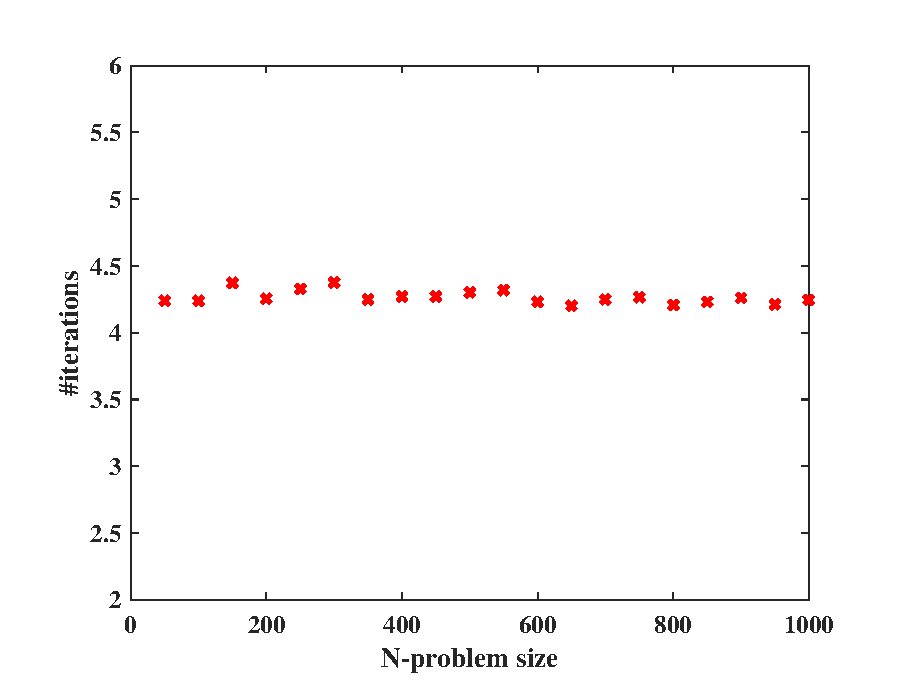
\includegraphics[scale=.7]{graphics/iters.eps}
\caption{A plot of iterations that the Gu-Eisenstat algorithm performs on average for finding the eigenvalue as problem size $N$ grows.}
\end{center}
\end{figure}
	
	Additionally, we tested the algorithm with various problem sizes and determined the complexity to be $O(\log(N))$ by performing a complexity analysis of run time and floating point operations. We ran our algorithm using randomly generated data of growing problem size $N$ and plotted the run time and flops as shown in Figure 2.

\begin{figure}
\begin{center}
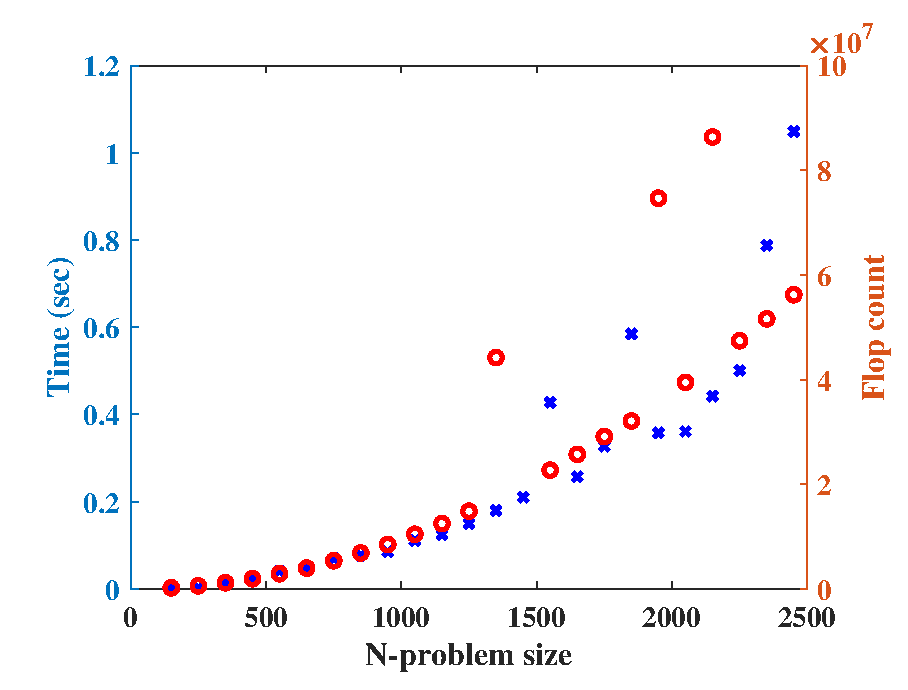
\includegraphics[scale=.7]{graphics/flops2500.eps}
\caption{A plot of the run time and floating point operation (flop) count of the Gu-Eisenstat algorithm for growing problem size $N$.}
\end{center}
\end{figure}	

\subsubsection*{2. Eigenvectors}
Computing the eigenvectors relies on knowing the eigenvalues. So, after we have read in our data and computed the final set of updated eigenvalues, we proceed to solve for eigenvectors. Consider we have $L = D - \Lambda$ where $D$ are the eigenvalues from the second to last Gu-Eisenstat run and $\Lambda$ is the final set of eigenvalues computed by Gu-Eisenstat. %To update the eigenvectors, we need to scale the new data point by a set of initially computed eigenvectors, let this update be $a = \frac{Q’}{l}$, where $Q'$ is the initial set of eigenvectors. 
%We can determine the updated eigenvectors by doing the following $Q = L v$ 
% further normalized via $$Q = \frac{Q^{\top}Q}{|Q|}.$$
 The updated eigenvectors are given by the system 
 \begin{equation}
 Q= \frac{S L^{-1} v}{\vert S L^{-1} v\vert} \ ,
 \end{equation}
where $S$ is the set of eigenvectors of the matrix $C_N$ and $v$ is the rank-1 update applied to the matrix $C_N$.
 
\subsubsection*{3. Adjustments to approach}
We faced floating point error with our eigenvalue solver. We would see this issue arise when using simulation data that had no noise.  As we received each update, the difference in eigenvalues from one update to the next would be so small, that over enough iterations, error would build up.  As of now, we have manually added noise to our simulation data.

	We also faced floating point error that occurred when we computed eigenvectors iteratively for each data point we received. This is because the difference between the eigenvectors before the update and after was so small, floating-point error would build up after various iterations. Therefore, we compute our eigenvectors after iteratively finding all eigenvalues using Gu-Eisenstat.


\section{DISCUSSION AND FUTURE WORK}
\label{disc}
As of now we have implemented rank-1 components that can be applied toward the building of a rank-1 dimensional reduction algorithm, such as a rank-1 PCA or rank-1 POD algorithm, however there are various ways we aim to refine and improve these components. 

Our data pipeline as of now uses randomly generated data and simulation data. As we have found with simulation data, there is need to add noise to avoid floating point errors. We aim to further examine how we can make our eigendecomposition algorithm robust to this issue. We aim to extend our data parser to read in data at a controlled rate, rather than reading in our data all at once. Additionally, we aim to implement a selective update routine wherein we would examine how a data point affects the eigenvalue decay of the eigendecomposition at that reading and determine whether to include that data point in our dimensionality reduction. This would allow for further improvements in memory usage by reducing the number of computations performed with new data points.

The rank-1 covariance algorithm as of now is mainly based on a PCA approach to dimensional reduction. We aim to expand this algorithm to be able to calculate the covariance matrix for use in POD based on the dimensionality of given data. For the eigendecomposition algorithm we would like to perform further testing on its performance on real-world data rather than just simulation data. Additionally, we would like to study how this algorithm could be reformulated to be parallelized onto GPUs to further improve its performance. Additionally, we would like to perform more extensive error checking of each component.

\section{ACKNOWLEDGEMENTS}
\label{ack}
This work was supported in part by the U.S. Department of Energy, Office of Science, Office of Workforce Development for Teachers and Scientists (WDTS) under the Science Undergraduate Laboratory Internships (SULI) program. 

Thank you to Oana Marin, for her unfaltering support and dedication to my experience this summer and beyond.  I also want to thank Jacob Freund, a fellow SULI student who collaborated with me on this project and Yuzhen Liu, for sharing her expertise and enthusiasm throughout the summer.

\bibliography{references} % Delete if no references
% See woc_2col.text for how to cite sources

 \begin{thebibliography}{9}
 %
 % and use \bibitem to create references.
 %

\bibitem{RefA}
van der Maaten, Laurens, Postma, Eric, and Herik, H., Dimensionality Reduction: A Comparative Review, Journal of Machine Learning Research, \textbf{10}

\bibitem{RefIntro}
Loong Chuen Lee, Abdul Aziz Jemain,
On overview of PCA application strategy in processing high dimensionality forensic data,
Microchemical Journal,
\textbf{169},
2021

\bibitem{RefB}
R. Mitz and Y. Shkolnisky, ROIPCA: An Online PCA algorithm based on rank-one updates, CoRR, (2019)

\bibitem{RefC}
D.M. Luchtenburg, B.R. Noack, and M. Schlegel, An introduction to the POD Galerkin method for fluid flows with analytical examples and MATLAB source codes, Berlin Institute of Technology MB1, Muller-Breslau-Strabe, \textbf{11}

\bibitem{RefBNS}
Bunch, J.R., Nielsen, C.P. , and Sorensen, D.C. Rank-one modification of the symmetric eigenproblem. Numer. Math. 31, 31–48 (1978)

\bibitem{RefD}
Gu, Ming and Eisenstat, Stanley C., A Stable and Efficient Algorithm for the Rank-One Modification of the Symmetric Eigenproblem,  SIAM Journal on Matrix Analysis and Applications, \textbf{15} (4), 1266-1276 (1994)

 \end{thebibliography}

\end{document}